%!TEX root = ../thesis.tex
% TODO: Change this?

\chapter{The \textit{IgH} locus in \textit{Nothobranchius furzeri}}  
\onehalfspacing

% Chapter summary (should fit on title page)

% Chapter 1 summary
% Should fit on chapter title page

\section*{Summary} % Fits one one page if 1.5-spaced, but not at double spacing


The turquoise killifish IgH locus resembles that of medaka, the most closely-related teleost species with a characterised \textit{IgH} locus, in several important respects, including an unusual IgM-TM splice pattern different from most teleosts and the absence of the teleost-specific antibody isotype IgZ/T. The shared absence of IgZ/T in these related species was particularly striking, as all previously-characterised teleost loci except medaka and grasscarp have been found to possess this isotype. Given their relatedness, it was hypothesised that \dots

\pagebreak

% Sections

\section{Introduction}

The structure of the immunoglobulin heavy chain (\textit{IGH}) locus defines the state space of antibody heavy-chain diversity and function in a species, determining both the V, D and J segments available for VDJ recombination and the range, structure and function of the possible antibody classes available to that organism. In addition to determining the possible antibody effector functions in a species, this locus is also responsible for the majority of diversity in antigen-specificity available to an organism, due to the exceptionally high diversity of the CDR3 junctional region compared to that of light chain loci. 

Determining the sequence and structure of the IGH locus in a species is therefore an essential step towards understanding and manipulating humoral adaptive immunity in a species, both in its own right and as an important stepping stone towards successful immunoglobulin sequencing in that taxon.

In addition to the instrumental importance of the IGH locus structure for immunoglobulin sequencing and other experimental interventions, however, it is also an important and interesting topic in its own right, revealing much about the functionality and evolution of antibody heavy chains in and between related species. In particular, while a number of IGH loci have been sequenced and characterised in the teleost fishes, these loci have been taken from a wide range of relatively distantly related species, chosen due to their use in agriculture or their prior status as experimental model organisms. There is therefore a lack of more closely-related loci that can be used to investigate the evolution of humoral immunity at higher temporal resolution. 

In this chapter, therefore, I present detailed characterisation of the IGH locus in the turquoise killifish, as well as that of another important model organism in the Cyprinodontiformes, namely the southern platyfish \textit{Xiphophorus maculatus}. In addition, I provide partial characterisations of loci from ten other cyprinodontiform species, with a focus on the constant-region exons and isotypes present across this important and diverse teleost clade. The results of these investigations demonstrate rapid evolution in the core functional components of humoral adaptive immunity within the cyprinodontiforms, with multiple independent losses of the IGHZ isotype and [something about CM and CD here]. These results raise exciting questions about the kinetics of immune-system evolution in this taxon and indicate the value of the cyprinodontiforms, and the African killifishes in particular, as a model for comparative evolutionary immunology in teleost fishes. 

\section{Materials and methods} % Maybe, maybe not, depends on final structure - maybe put relevant stuff here for draft and then move it later?

\dots
\pagebreak



\section{The \textit{IgH} locus in \textit{Nothobranchius furzeri}}
\label{sec:nfu-locus}


	\subsection{Overall structure}
	\label{sec:nfu-locus-structure}
	
	The turquoise killifish genome contains a single \textit{IgH} locus approximately 305 kilobases in length, located towards the 3' end of chromosome 6 (\Cref{fig:nfu-locus-map-a}).
	This locus comprises two complete subloci, IGH1 (155 kb) and IGH2 (118 kb), present in tandem and each occupying a classic ${VH-DH-JH-CH}$ translocon configuration. This modified translocon structure, with multiple translocon subloci present in tandem, has been observed in a number of teleost \textit{IgH} loci including catfish, medaka and stickleback. Unusually, however, the smaller IGH2 sublocus in TK \textit{IgH} is present in antisense relative to the larger IGH1, with the two subloci beginning at opposite ends of the locus and facing each other in the middle (\Cref{fig:nfu-locus-map-b}). Such a multi-orientation locus structure has only previously been observed in medaka, and there only in a small, partially-assembled sublocus of uncertain functionality; it is interesting to see this unusual feature reproduced here, in a fairly closely-related species, and it is possible that this ideosyncracy is homologous between the two loci. % TODO: Use RNA-seq data to check functionality of IGH2
	
	Compared to other closely-related loci, the killifish locus is relatively sparse and simple, with comparatively low functional complexity relative to its overall size. For example, whereas the stickleback locus fits four subloci, 49 V segments and 10 constant regions into c. 200 kb, the killifish locus, despite being ~50\% longer, contains only 2 subloci, four constant regions and 24 V segments (including pseudogenised Vs). This difference results from the unusually large amount of nonfunctional sequence padding the killifish locus, resulting in large gaps between variable segments and in some cases between constant-region exons (\Cref{fig:nfu-locus-map-b}); this high prevalence of repetitive DNA is consistent with the rest of the TK genome, which comprises more than 60\% repetitive sequence, compared to just over 15\% in stickleback.
	
	The two subloci in the turquoise killifish locus are generally highly similar in their functional sequence, with a high degree of synteny between their functional regions (\Cref{fig:nfu-locus-synteny}). The greatest degree of divergence occurs in the VH and DH regions, with what appear to be repeated deletion events in IGH2 resulting in a substantially lower number of VH and DH segments compared to IGH1; conversely, the JH and constant regions are almost identical between two subloci. These patterns are discussed in more detail in \Cref{sec:nfu-locus-constant,sec:nfu-locus-variable}.
	
	% TODO: How can I distinguish between deletions in IGH2 and insertions in IGH1?
	% TODO: Can I say anything about the history of the locus? Ask David.
	
	\begin{figure}
	\centering
	\includegraphics[width=\textwidth]{/home/will/Documents/code/figures/2018-11-06/nfu-locus-map_small} % TODO: Move to thesis directory, switch to large figure
			    \begin{subfigure}{0em}
        \phantomsubcaption{}
        \label{fig:nfu-locus-map-a}
    \end{subfigure}
    \begin{subfigure}{0em}
        \phantomsubcaption{}
        \label{fig:nfu-locus-map-b}
    \end{subfigure}
    \begin{subfigure}{0em}
        \phantomsubcaption{}
        \label{fig:nfu-locus-map-c}
        \end{subfigure}
	\caption[The immunoglobulin heavy chain (\textit{IGH}) locus in \textit{Nothobranchius furzeri}]{\textbf{The immunoglobulin heavy chain (\textit{IgH}) locus in \textit{Nothobranchius furzeri}:} (A) Position of the \textit{IgH} locus on chromosome 6 of the \textit{N. furzeri} genome. (B) Arrangement of VH, DH, JH and constant-region gene segments on the \textit{N. furzeri} \textit{IgH} locus. All segments follow the orientation of their parent sublocus, indicated in the uppermost track. (C) Detailed map of the constant regions of the \textit{IGH1} sublocus, indicating the position and identity of the constant-region exons and the exon composition of expressed \textit{IgH} isoforms in the turquoise killifish.}
	\label{fig:nfu-locus-map}
	\end{figure}
	
	\begin{figure}
	\centering
	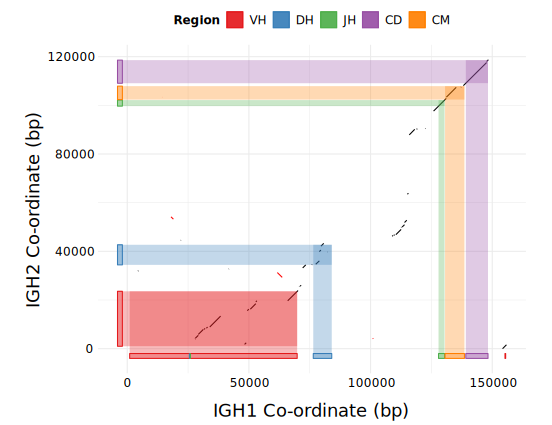
\includegraphics[width=0.9\textwidth]{_Figures/png/nfu-locus-dots.png}
	\caption[Sequence homology between subloci in \textit{N. furzeri} \textit{IGH}]{\textbf{Sequence homology between subloci in \textit{N. furzeri} \textit{IGH}:} Synteny plot of sequential best matches between \textit{IGH1} and \textit{IGH2} subloci, with gene segment regions indicated by coloured rectangles along each axis.}
	\label{fig:nfu-locus-synteny}
	\end{figure}
	
	\subsection{Constant regions}
	\label{sec:nfu-locus-constant}
	
	The isotype (also known as the class) of an antibody determines its functional role within the immune system, including its possible effector functions and whether it can be secreted. Three antibody isotypes have been identified to date in teleost fishes: IgM, IgD and IgZ (a.k.a. IgT, IgT/Z or IgZ/T). Of these, IgM and IgD are highly primitive within the jawed vertebrates and found in most or all other vertebrate groups; within the teleosts, both appear to be universal. Conversely, IgZ is a teleost-specific isotype which is absent in other vertebrate taxa; within the teleosts, most characterised exons possess IgZ, but at least two (medaka and channel catfish) have been found to lack it. In rainbow trout, IgZ has been found to play a specialised mucosal role in the immune system analagous to that of IgA in mammals, and it is widely assumed to play this specialised role throughout the teleosts; it is as yet unclear how mucosal immunity is effected in species lacking IgZ.
	
	IgM, the most primitive and widely-found isotype in jawed vertebrates, is present immediately downstream of the main JH-region and occupies the standard six-exon configuration, with four \cm{} exons and two transmembrane domains present in series on the chromosome (\Cref{fig:nfu-locus-map-b,fig:nfu-locus-map-c,fig:teleost-igm-exons-a}). As with other species, both secreted and transmembrane isoforms of IgM are present in the transcriptome, with secreted IgM consisting of \cm{1-4} (\Cref{fig:nfu-locus-map-c,fig:nfu-locus-sashimi-a,fig:teleost-igm-exons-b}); however, the exon configuration of transmembrane IgM deviates from both that seen in mammals (in which exon TM1 is spliced to a cryptic splice site within \cm{4}) and most teleosts (in which the canonical splice site following \cm{3} is used and \cm{4} is excised). Rather, TK IgM-TM resembles that of medaka, in which both \cm{3} and \cm{4} are excluded and the canonical splice site at the end of \cm{2} is spliced directly to TM1 (\Cref{fig:teleost-igm-exons-c,fig:teleost-igm-exons-d,fig:teleost-igm-exons-e}). The similarity to medaka, which again is the closest relative of TK with a characterised locus, raises the possibility that this unusual splicing behaviour may be a conserved feature of both lineages; however, the underlying mechanism giving rise to this difference in splicing behaviour is unknown.
	
		Unlike IgM, the exon structure of IgD is highly variable across the teleosts, ranging from roughly 7-17 \cd{} exons in addition to the transmembrane domains. The core structure of IgD comprises seven \cd{} exons (\cd{1-7}), but some subset of these exons may be missing or duplicated in any given species -- in medaka, for example, \cd{5} is missing in all subloci, while in many species (e.g. zebrafish, salmon, and channel catfish) \cd{2-4} are duplicated in two or more tandem blocks. This latter configuration is a in turquoise killifish, in which the IgD constant region immediately follows IgM in both subloci and has a 

\cd{1}-(\cd{2}-\cd{3}-\cd{4})$_2$-\cd{5}-\cd{6}-\cd{7}-TM1-TM2 

	\noindent configuration, for a total of 12 exons per IgD constant region (\Cref{fig:nfu-locus-map-b,fig:nfu-locus-map-c}). All of these exons appear to be expressed in tandem, resulting in a much longer IgH transcript than is observed for any isoform of IgM (\Cref{fig:nfu-locus-map-c,fig:nfu-locus-sashimi-b}). Of the duplicated exon pairs, \cm{3}A/B and to a lesser extent \cm{4}A/B are highly similar, while \cm{2}A/B are more distinct (\Cref{fig:nfu-ch-aln}). As in other teleost species, IgD in the turquoise killifish includes a chimeric \cm{1} exon at the 5' end of the constant-region transcript, for a total of 13 exons per IgD-TM mRNA (\Cref{fig:nfu-locus-sashimi-b}).

	While the best-known form of IgD in teleosts is transmembrane, secreted IgD has been observed in at least two teleost species, with different mechanisms used in each case: in channel catfish, one dedicated sublocus has a dedicated IgD secretory exon in place of the transmembrane exons, while in rainbow trout (and possibly some other species like Atlantic salmon and cod) a run-on event at the end of \cd{7} results in the production of a secretory tail in a manner similar to secretory IgZ. However, neither a specialised secretory exon nor a \cd{7} secretory tail could be detected in turquoise killifish, suggesting that IgD may only be expressed in transmembrane form in this species. % TODO: Figure comparing post \cd{7} sequence in trout, salmon, cod and TK (and other species from paper?) to demonstrate lack of secretory tail in TK
	
	In the case of both IgM and IgD, the constant regions are present in their expected configuration in each sublocus and are highly similar in sequence between the subloci, with an average of 98.4\% nucleotide sequence identity for corresponding IgM exons and 99.3\% for corresponding IgD exons (\Cref{fig:nfu-ch-aln} and \Cref{tab:nfu-ch-aln}).

	The most striking feature of the constant-region structure of the \textit{IGH} locus in \textit{N. furzeri} is the complete absence in both subloci of IgZ. As discussed above, IgZ constant exons have been found to be present in the great majority of teleost \textit{IgH} loci characterised to date, with the only previous exceptions being channel catfish and medaka. Its absence in turquoise killifish (\Cref{fig:nfu-locus-map-b}) is therefore notable, and immediately raises questions about the nature, kinetics and efficacy of mucosal adaptive immunity in this species. Since medaka, the closest relative of TK with a characterised locus, also lacks IgZ, its absence in TK also raises the question of whether its absence occurred in a common ancestor to both species or is the result of independent deletion events in both lineages; this question is addressed in more depth in subsequent sections of this chapter. % IgZ paragraph at start or end of subsection?	
	
	% TODO: I need to do an amino-acid sequence alignment to reference species here so I can actually get percentage identity numbers (plus it will make a nice figure), but the identity with other teleost species at each exon seems quite high.
	

	% TODO: Table and figure of antibody isoforms in TK: length, molecular weight, number of C-regions, etc. (in appendix)
	
	\begin{figure}
	\centering
		    \begin{subfigure}{0em}
        \phantomsubcaption{}
        \label{fig:teleost-igm-exons-a}
    \end{subfigure}
    \begin{subfigure}{0em}
        \phantomsubcaption{}
        \label{fig:teleost-igm-exons-b}
    \end{subfigure}
    \begin{subfigure}{0em}
        \phantomsubcaption{}
        \label{fig:teleost-igm-exons-c}
    \end{subfigure}
    \begin{subfigure}{0em}
        \phantomsubcaption{}
        \label{fig:teleost-igm-exons-d}
    \end{subfigure}
    \begin{subfigure}{0em}
        \phantomsubcaption{}
        \label{fig:teleost-igm-exons-e}
    \end{subfigure}
	\includegraphics[width=0.8\textwidth]{_Figures/png_edited/teleost-igm-exons}
	\caption[IgM exon usage in other vertebrates]{\textbf{IgM exon usage in other vertebrates:} Schematic of IgM splice patterns in different isoforms and taxonomic groups; (A) standard genomic (pre-splicing) configuration of IgM, following VDJ recombination; (B) exon configuration of secreted IgM (IgM-S) in tetrapods and teleosts; (C) exon configuration of transmembrane IgM (IgM-TM) in tetrapods, demonstrating the use of a cryptic splice site in \cm{4}; (D) standard IgM-TM exon configuration in teleosts, demonstrating the direct splicing of \cm{3} to TM1 and exclusion of \cm{4}; (E) unusual IgM-TM exon configuration observed in medaka, in which both \cm{3} and \cm{4} are excluded. Figure adapted from Fillatreau \textit{et al.} (2013).}
	\label{fig:teleost-igm-exons}
	\end{figure}
	
	\begin{figure}
	\centering
			    \begin{subfigure}{0em}
        \phantomsubcaption{}
        \label{fig:nfu-locus-sashimi-a}
    \end{subfigure}
    \begin{subfigure}{0em}
        \phantomsubcaption{}
        \label{fig:nfu-locus-sashimi-b}
    \end{subfigure}
	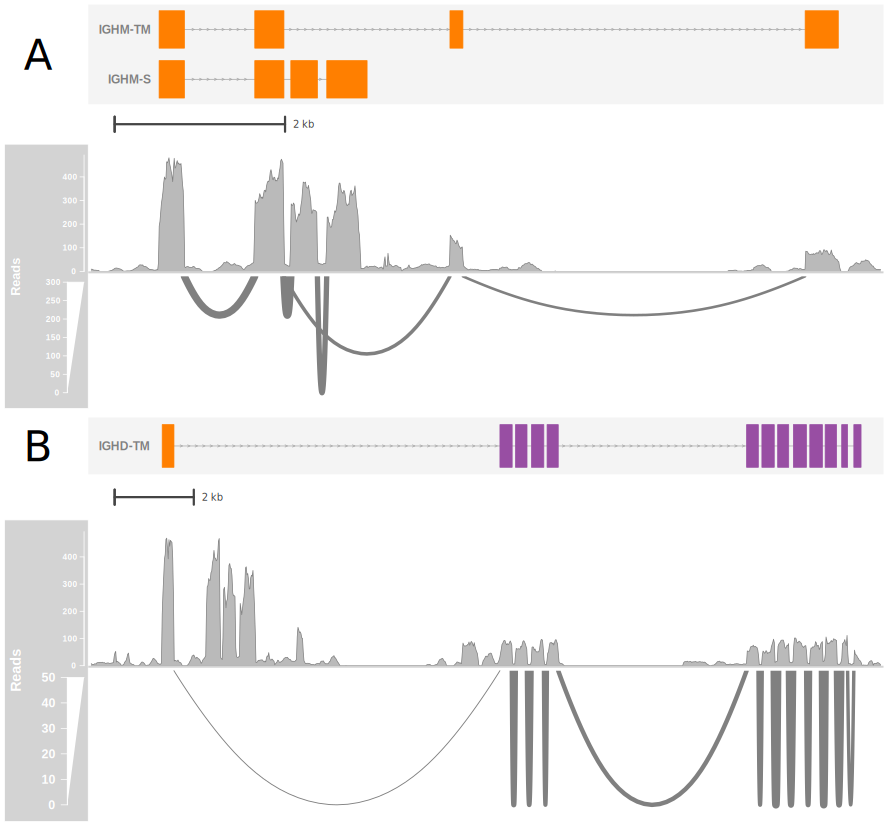
\includegraphics[width=\textwidth]{_Figures/png/nfu-locus-sashimi}
	\caption[Constant-region isoforms in \textit{N. furzeri}]{\textbf{Constant-region isoforms in \textit{N. furzeri}:} Coverage and sashimi plots of STAR-aligned RNA-seq reads from \textit{N. furzeri} gut samples, demonstrating the splicing behaviour of IGH1 constant-region isoforms. (A) IGHM exon splicing, showing alternative splicing patterns of IGHM-TM and IGHM-S; (B) IGHD exon splicing, including splicing of \cm{1} to \cd{1}.}
	\label{fig:nfu-locus-sashimi}
	\end{figure}
	
	\begin{figure}
	\centering
	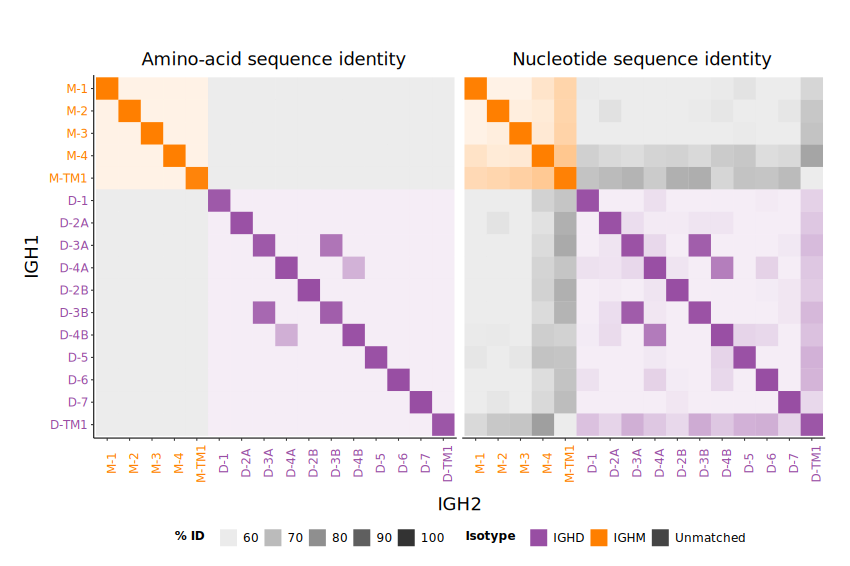
\includegraphics[width = \textwidth]{_Figures/png/nfu-ch-aln}
	\caption[Cross-sublocus sequence similarity in constant-region exons in \textit{N. furzeri} \textit{IGH}]{\textbf{Cross-sublocus sequence similarity in constant-region exons in \textit{N. furzeri}:} Heatmap of percentage sequence identity between amino-acid (right) and nucleotide (left) sequences of constant-region exons from the two subloci of \textit{N. furzeri} \textit{IGH}, calculated using pairwise Needleman-Wunsch global alignments. Note the very high similarity between corresponding exons of the two subloci, as well as the substantial similarity between IGHD-3A/3B and IGHD-4A/4B in both subloci.}
	\label{fig:nfu-ch-aln}
	\end{figure}
	
	\begin{table}\centering
		\caption[Cross-sublocus sequence similarity between corresponding constant-region exons in \textit{N. furzeri} \textit{IGH}]{\textbf{Cross-sublocus sequence similarity in constant-region exons in \textit{N. furzeri}:} Percentage sequence identities of pairwise Needleman-Wunsch global alignments between nucleotide (NT) or amino-acid (AA) sequences of corresponding exons from the two subloci of \textit{N. furzeri} \textit{IGH}.}
	% latex table generated in R 3.5.1 by xtable 1.8-3 package
% Wed Nov 21 11:59:38 2018
\begin{tabular}{llrr}
  \toprule Isotype & Exon & NT & AA \\ 
  \midrule M & 1 & 99.66 & 100.00 \\ 
  M & 2 & 100.00 & 100.00 \\ 
  M & 3 & 100.00 & 100.00 \\ 
  M & 4 & 100.00 & 100.00 \\ 
  M & TM1 & 99.34 & 98.00 \\ 
  M & TM2 & 91.67 & 100.00 \\ 
  D & 1 & 99.03 & 97.06 \\ 
  D & 2A & 98.97 & 98.96 \\ 
  D & 3A & 98.72 & 97.09 \\ 
  D & 4A & 99.65 & 98.92 \\ 
  D & 2B & 100.00 & 100.00 \\ 
  D & 3B & 98.72 & 96.12 \\ 
  D & 4B & 99.64 & 98.91 \\ 
  D & 5 & 99.09 & 99.08 \\ 
  D & 6 & 100.00 & 100.00 \\ 
  D & 7 & 100.00 & 100.00 \\ 
  D & TM1 & 97.99 & 97.96 \\ 
  D & TM2 & 99.44 & 100.00 \\ 
   \bottomrule \end{tabular}

	\label{tab:nfu-ch-aln}
	\end{table}
	




	\subsection{Variable regions}
	\label{sec:nfu-locus-variable}
	
	\subsubsection{Organisation, functionality and diversity}
	\label{sec:nfu-locus-variable-orga}
	 
	% Presence and functionality
	In total, 24 VH-segments, 14 DH-segments and 17 JH-segments were identified in the \textit{N. furzeri} locus, of which the majority (17 VH, 10 DH and 8 JH) were present in \textit{IGH1}. Of the VH segments identified, three contain premature STOP codons, though none is out-of-frame; conversely, all the DH and JH segments identified appear to be in-frame and functional, with no premature STOP codons. However, in all cases a minority of segments contain RSS sequences that deviate significantly from the expected consensus sequence; it is unclear whether these sequences can recombine to successfully produce mature VDJ sequences \textit{in vivo}. In the case of the VH segments, of the six sequences without clearly functional RSS sequences, three also contain premature STOP codons, suggesting the changes to the RSS in these cases may arise from relaxed purifying selection on already-pseudogenised sequences.
	
	% Location and exceptions
	Of the VH, DH and JH segments identified, all but one of each type of segment is located within contiguous V-, D-, and J-regions within each sublocus, supporting a modified translocon configuration for killifish \textit{IGH}. The exceptions to this are IGH1D01 and IGH1J01, which are embedded within the IGH1 V-region, and a single VH segment located in between the IGHD contant regions of the two subloci (\Cref{fig:nfu-locus-map-b}). The unusual location of IGH1D01 and IGH1J01 may represent the result of a transposition event within the IGH locus; however, their close colocalisation and 5' position within the IGH1 sublocus, as well as the fact that neither has a close paralogue in IGH2 (\Cref{fig:nfu-dj-alignment-b}), suggest that they may alternatively represent the remnant of a formerly present IGHZ constant region, as these typically have dedicated D/J segments independent of those serving IGHM. Given its forward orientation, meanwhile, the orphaned VH-segment was assigned to the IGH1 sublocus as IGH1V1-07; however, if annotated correctly, it is unlikely to successfully recombine with segments in either sublocus due to its unusual location. % Alternatively, the unusual location of this VH segment could be due to either a misassembly or the presence of an additional sublocus missing from the current assembly; however, given the structurally volatile nature of the IGH locus and the frequency with which isolated VH loci are found in other parts of the genome, the presence of an orphaned locus in between two functional subloci is not implausible.
		
	% Segment numbers
	The total number of functional VH segments in the killifish locus is unusually small in comparison to the total numbers observed in many other teleost species (\Cref{tab:teleost-vh-counts}); however, the number of segments per sublocus is in line with the numbers seen in closely-related species (2 to 12 in medaka, 6 to 18 in stickleback), with the overall difference mainly arising from a difference in the number of subloci per locus. A similar pattern is observed with DH and JH segments, with similar numbers of segments per sublocus in killifish and closely-related species, especially medaka. It therefore appears that the per-sublocus segment diversity available to the turquoise killifish is similar to that of previously characterised species, with any difference in total available diversity at this level arising from differences in the number of functional subloci rather than the size of the V/D/J-regions \textit{per se}. % TODO: Compute total number of possible VDJ combinations compared to other species?
	
	\begin{table}
	\begin{threeparttable}
	\caption{\textbf{Number of functional VH-segments and VH-families in other teleost species}}
	\label{tab:teleost-vh-counts}
	\begin{tabular}{ccccc}\toprule
	\textbf{Common Name} & \textbf{Species} & \textbf{\# Functional VH Segments} & \textbf{\# VH Families} & \textbf{Source}\\\midrule
	Zebrafish & \textit{Danio rerio} & 39 & 13\,\tnote{1} & Magadan 2015 \\
	Grasscarp & \textit{Ctenopharyngodon idella} & 8 & 5\,\tnote{2} & Xiao 2010 \\
	Fugu & \textit{Takifugu rubripes} & 34 & 3 & Magadan 2015 \\
	Medaka & \textit{Oryzias latipes} & 35 & 6 & Fillatreau, Magadan 2011 \\
	Stickleback & \textit{Gasterosteus aculeatus} & 49 & 4 & Magadan 2015 \\
	Turquoise killifish & \textit{Nothobranchius furzeri} & 21\,\tnote{3} & 6 & -- \\
	\bottomrule\end{tabular}
	\begin{tablenotes}
	\item[1] VH families in zebrafish identified based on 70\% (rather than 80\%) sequence identity.
	\item[2] It is not clear what clustering method or threshold was used to identify VH families in grasscarp.
	\item[3] Excluding VH segments with nonsense or frameshift mutations, but not those with uncertain or missing RSS sequences.
	\end{tablenotes}
	\end{threeparttable}
	\end{table} % TODO: Convert source labels into proper citations
	
	\subsubsection{Sublocus synteny and evolution}
	\label{sec:nfu-locus-variable-synteny}

	% Synteny
		As can be seen from \Cref{fig:nfu-locus-synteny}, much of the V-, D- and especially J-region sequence in the \textit{N. furzeri} locus is syntenic between the two \textit{IGH} subloci, with downstream portions of the \textit{IGH2} V-region corresponding to downstream parts of the \textit{IGH1} region (after correcting for locus orientation). Of the seven VH segments in \textit{IGH2}, six have a correspending segment on \textit{IGH1} with which they share at least 97\% sequence identity (\Cref{fig:nfu-vh-families}), and these partner segments are largely (but not entirely) colinear in their ordering between the two subloci. A similar pattern can be observed for the D- and (especially) the J-regions: of the four DH segments detectable in IGH2, three (IGH2D02 to IGH2D04) are identical with another block of adjacent DH segments in IGH1 (IGH1D05 to IGH1D07), while the the J-regions exhibit almost complete sequence identity between the eight JH segments of the main JH region in IGH1 and the eight JH segments in IGH2 (\Cref{fig:nfu-dj-alignment}).
		
		Nevertheless, as is clear from \Cref{fig:nfu-locus-synteny}, there are large portions the \textit{IGH1} variable region, including the first 25 kilobases of the V-region, for which no corresponding sequence exists in \textit{IGH2}, and there are many VH and DH segments in IGH1 (and a much smaller number in IGH2) for which no close homologue exists in the other sublocus. Taken together, these data are consistent with a model in which \textit{IGH2} was produced via duplication and inversion of all or part of \textit{IGH1}, followed by subsequent deletion events in the redundant, and structurally volatile, \textit{IGH2} VH and DH regions. However, it is not clear at present how to distinguish between this model and an alternative one of expansion in IGH1, explain why IGH2 and IGH1 should have undergone deletion events, or identify why the JH region is so much more conserved between subloci than either the VH or JH regions.
% TODO: Think about these questions, try to suggest hypotheses
		

	\subsubsection{VH families}
	\label{sec:nfu-locus-variable-families}
	
	VH sequences within an \textit{IGH} locus are conventionally grouped into families on the basis of nucleotide sequence identity, with a typical identity cutoff of 80\%. In order to group the \textit{N. furzeri} VH genes into families, pairwise Needleman-Wunsch global alignments were performed on each pair of VH sequences to obtain pairwise identity scores, followed by single-linkage clustering on the resulting identity matrix. Cutting the dendrogram at 80\% sequence identity revealed a total of six VH families, of which four contained more than one VH segment (\Cref{fig:nfu-vh-families}). 	V2 and V4 are highly similar and all the members of V4 are pseudogenised by premature STOP codons; it may therefore be better to regard V4 as a pseudogenised subfamily of V2 than a VH family in its own right. Of the remaining families, V1 and V2 make up the bulk (42\% and 29\% respectively) of the VH segments in the locus. 
	
	The number of VH families is roughly in line with those found in related species (\Cref{tab:teleost-vh-counts}), indicating that, while the total number of VH segments in the turquoise killifish may be unusually low (see \Cref{sec:nfu-locus-variable-orga}), the degree of sequence diversity found \textit{among} these segments is in line with other, previously-characterised teleost species. 
	
	\begin{figure}
	\centering
	\begin{subfigure}{0em}
	\phantomsubcaption{}
    \label{fig:nfu-vh-families-a}
    \end{subfigure}
    \begin{subfigure}{0em}
    \phantomsubcaption{}
    \label{fig:nfu-vh-families-b}
    \end{subfigure}
	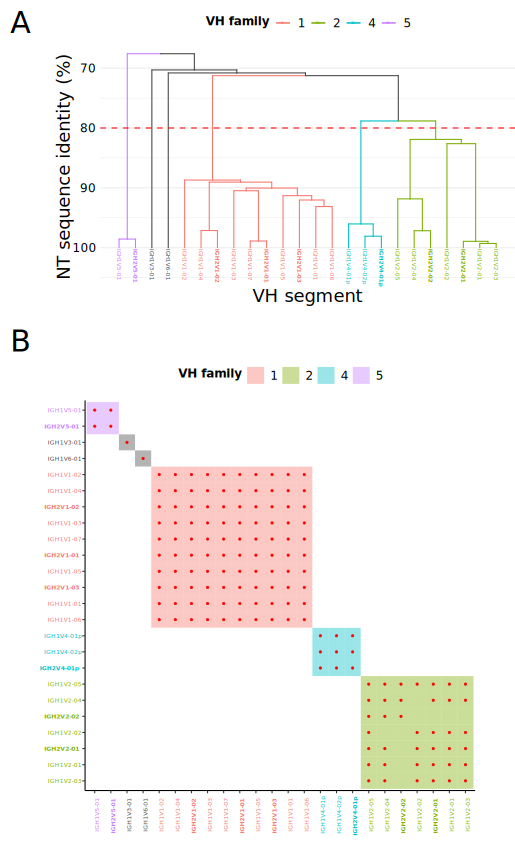
\includegraphics[width=0.8\textwidth]{_Figures/png/nfu-vh-families.png}
	%\includegraphics[width=\textwidth]{/home/will/Documents/code/figures/2018-11-08/nfu-vh-families_small} % TODO: Move to thesis directory, switch to large figure
	\caption[VH families in the in \textit{N. furzeri} \textit{IgH} locus]{\textbf{VH families in the in \textit{N. furzeri} (\textit{IgH}) locus:} (A) Dendrogram of sequence similarity of VH segments in the \textit{N. furzeri} locus, arranged by single-linkage clustering on nucleotide sequence identity. The red line indicates the 80\% cutoff point for family assignment, while branch colour indicates family membership. (B) Heatmap of family relationships among \textit{N. furzeri} VH segments, with coloured shading indicating families and red dots indicating pairwise nucleotide sequence identity of at least 80\%. In both subfigures, VH families containing multiple segments are coloured, single-segment families are in grey, and segments from the IGH2 sublocus are displayed in \textbf{boldface}.}
	\label{fig:nfu-vh-families}
	\end{figure}

	% TODO: Detailed V-co-ordinate table (in appendix)	

\begin{figure}
\centering
	\centering
	\begin{subfigure}{0em}
	\phantomsubcaption{}
    \label{fig:nfu-dj-alignment-a}
    \end{subfigure}
    \begin{subfigure}{0em}
    \phantomsubcaption{}
    \label{fig:nfu-dj-alignment-b}
    \end{subfigure}

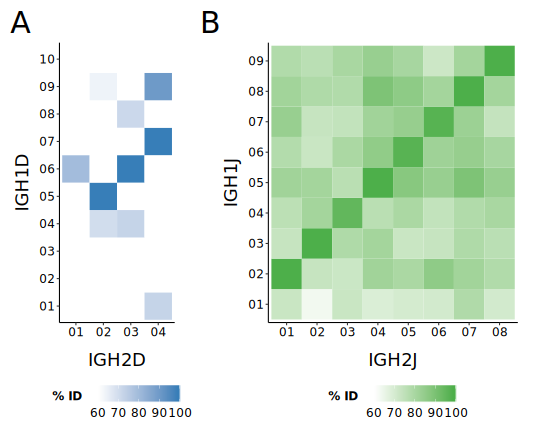
\includegraphics[width=0.6\textwidth]{_Figures/png/nfu-dj-aln}
\caption[Cross-sublocus sequence similarity in DH and JH gene segments in \textit{N. furzeri}]{\textbf{Cross-sublocus sequence similarity in DH and JH gene segments in \textit{N. furzeri}:} Heatmap of percentage nucleotide sequence identities of Needleman-Wunsch global alignments between (A) DH and (B) JH gene segments in IGH1 vs IGH2, revealing syntenic runs of highly similar sequences across both subloci.}
\label{fig:nfu-dj-alignment}
\end{figure}

	\subsubsection{Recombination signal sequences}
	
	In their heptamer sequences, nonamer sequences, and spacer lengths, the recombination signal sequences (RSS) marking the ends of the VH, DH and JH gene segments in the \textit{N. furzeri} locus strongly resemble those of other characterised teleosts, which in turn match those of non-teleost loci (\Cref{fig:nfu-rss-seqlogo-all}). The overall heptamer and nonamer consensus sequences (\texttt{CACAGTG} for heptamers and \texttt{ACAAAAACC} for nonamers) closely matched those expected from the literature, while in 88\% of cases the spacer region was within 1bp of the expected length (12bp for D-RSSs, 23bp for V- and J-RSSs); unexpectedly, the greatest number of VH-RSSs had a 22bp (rather than 23bp) spacer, but this is not expected to interfere with RSS functionality. Overall, the RSSs in the turquoise killifish appear to be supporting the normal operation of VDJ-recombination in this species.
	
	\begin{figure}
	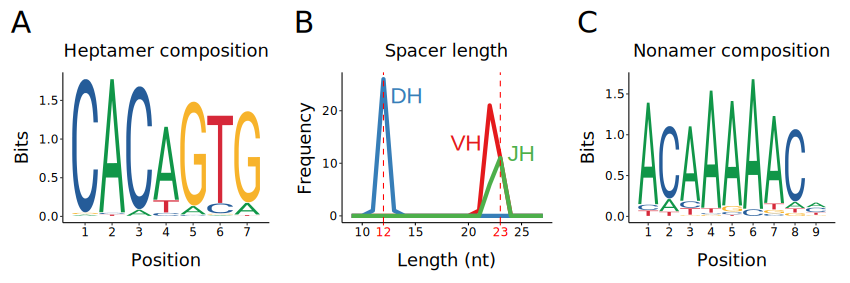
\includegraphics[width=\textwidth]{_Figures/png/nfu-rss-seqlogo-all}
	\caption[Recombination signal sequences in the \textit{N. furzeri} \textit{IGH} locus]{\textbf{Recombination signal sequences in the \textit{N. furzeri} \textit{IGH} locus:} (A) Sequence composition of conserved heptamer sequences across all \textit{N. furzeri} heavy-chain RSSs; (B) length distribution of unconserved spacer sequences in \textit{N. furzeri} heavy-chain RSSs; (C) sequence composition of conserved heptamer sequences across all \textit{N. furzeri} heavy-chain RSSs.}
	\label{fig:nfu-rss-seqlogo-all}
	\end{figure} % TODO: Add in row showing expected consensus sequence with highlighted conserved positions
	
	
	% TODO: Killifish V/D/J RSS sequence logos (separately, in appendix)



	
	\subsection{Discussion}
	
	The turquoise killifish IGH locus shares many features with other characterised teleost loci, including a modified tandem-translocon configuration with intact V, D, J and constant regions, six-exon secreted configuration of immunoglobulin M, expanded IgD constant region with tandem \cd{}-exon block repeats, conserved RSS structure, chimeric \cm{1} in IGHD, et cetera. However, it also exhibits many ideosyncratic features that differ from those observed in most characterised teleost loci, including an unusually small number of VH segments, a four-exon \cm{1}-\cm{2}-TM1-TM2 configuration of transmembrane IgM, an inverted sublocus present in antisense, and a complete absence of immunoglobulin Z. 
	
	Many of these peculiarities, including the unusual IgM-TM splicing pattern, inverted sublocus, and lack of IgZ, are shared with the sublocus of medaka (\textit{Oryzias latipes}), which until the completion of this study was the closest relative of \textit{Nothobranchius furzeri} to have its immunoglobulin heavy chain locus characterised. Given this close relationship between turquoise killifish and medaka, an obvious hypothesis for the evolutionary history of these unusual traits was of a common origin in the common ancestor of the Cyprinodontiformes (the clade that contains the killifishes) and the Beloniformes (the clade that contains medaka). % Tree for this 

	To investigate this hypothesis, I performed a complete characterisation of the \textit{IgH} locus in the platyfish \textit{Xiphophorus maculatus}, another cyprinodontiform species that has seen widespread use as a model organism. Alongside this, I performed a more limited characterisation of the \textit{IgH} constant regions in 9 %?
	additional cyprinodontiform species, to assess the broader patterns of immunoglobulin heavy chain evolution within this diverse and important teleost clade.
	
	% TODO: Relationship between killifish Vs and other species
	% TODO: Evolution of IGH1 vs 2
	% TODO: Discussion of mucosal immunity in absence of IGZ
		% TODO: Discuss smallness of killifish locus in the context of relaxed purifying selection and short life span
	% TODO: Section on "Investigating the evolutionary relationship between IGH1 and IGH2"
	% Keep for discussion:
%\q{Given the lack of IgZ in this species, how do you think they carry out mucosal immunity?}
%
%I'd assume using IgM. It's the primitive antibody and is expressed in secreted form in the killifish gut. I haven't investigated the protein expression so it's hard to say for sure, but I'd guess that's the answer. It's also quite possible, lacking a specialised mucosal class, that the answer is ``not very well". It would be very interesting to compare mucosal immune function in species with and without IgZ, especially if those species are closely related.
%
%Given the impressive results indicating the specificity of IgT for mucosal immunity in trout, and the lack of mucosal response of IgM in that species, it would be very interesting to see what mucosal responses look like in a species that lacks that isotype -- is IgM much more responsive and expressed in the gut than in IgT-possessing species, or is the mucosal response just worse?
	% (Incidentally, it would be great to see whether any B-cells in TK show recombinations in both subloci, vs one or the other. Single-cell DNA sequencing could plausibly do this.)



\section{The \textit{IgH} locus in \textit{Xiphophorus maculatus}}

	\subsection{Overall structure}
	
	The \textit{X. maculatus} \textit{IGH} locus occupies roughly 263 kb on chromosome 16, in a region syntenic with chromosome 6 of the \textit{Nothobranchius furzeri} genome. % TODO: Get a synteny plot of this, based on David's data.
	The \textit{X. maculatus} \textit{IGH} locus differs from the \textit{N. furzeri} locus in several important respects: % List them here first, then arrange them into prose
	\begin{itemize}
	\item Unlike the \textit{N. furzeri} locus, the \textit{X. maculatus} locus contains only a single sublocus spanning the entire length of the locus, with no evidence of a second, antisense sublocus as seen in \textit{N. furzeri}.
	\item The V-region of the \textit{X. maculatus} locus is highly expanded, with 99 identified VH segments -- more than four times the total number seen in \textit{N. furzeri}, and almost six times the number in the largest \textit{N. furzeri} sublocus. At least 74 of these VH segments appear to be fully in-frame and functional and equipped with functional RSS sequences, representing one of the highest numbers of functional VH segments seen in any teleost IGH locus. However, the final four VH segments (of which two are structurally intact) are downstream of the last identified DH segment and inverted relative to the rest of the locus, and may not be able to successfully undergo VDJ recombination. These VH sequences are also much more tightly packed than in the \textit{N. furzeri} locus, consistent with a lower overall prevalence of repetitive regions in the \textit{X. maculatus} genome. % TODO: Citation and number needed
	\item Unlike the turquoise killifish, the platyfish locus contains a fully intact IGHZ constant region, with a six-exon structure homologous with that seen in most other teleost loci (though not stickleback, in which the exon corresponding to \cz{2} is missing) and a secretory tail produced by a run-on event from \cm{4}. As in most teleost loci, this IGHZ constant region has its own dedicated DH and JH regions, though these are unusually small with only a single IGHDZ01 and IGHJZ01 segment each. % TODO: Compare these to the orphaned D/J segments in TK to test vestigial IGHZ hypothesis
	Unlike most IGHZ-bearing teleost loci, however, the \textit{X. maculatus} IGHZ constant region is upstream of the great majority of VH segments in the locus, with only one VH segment upstream of the \cz{1} exon. This lone VH segment, IGHV01-01, is distinct in sequence from the other VH segments in the locus, but appears to be functional. It would be interesting to see whether it (a) forms the expected invariant VDJ combination in recombined IGHZ transcripts, (b) can recombine with downstream DH segments to form part of recombined IGHM/D-specific transcripts. % TODO: Characterise IGHZ splicing, secreted vs transmembrane expression, etc.
	\item Rather than a single, relatively densely-packed D-region, the \textit{X. maculatus} locus contains DH segments interspersed throughout the long stretch of the locus between the end of the \textit{IGHZ} constant region and the start of that of IGHM. Many of these lone DH segments are closely associated with single JH segments, raising the possibility of a more cluster-like behaviour in which each $V_n-D_1-J_1$ group acts as a distinct recombination unit. However, the presence of a dense eight-segment J-region immediately upstream of IGHM, combined with a pair of comparatively closely-packed DH segments downstream of the last forward-oriented VH segments, suggests a more conventional translocon behaviour; it remains to be seen which of these traditional models of antigen-receptor structure more closely matches the in vivo recombination behaviour of this unusually structured IGH locus.
	% TODO: See if you can get any information on VDJ recombination patterns from Xiphophorus RNA-seq data
	% TODO: Assess RSS structure in platyfish
	% TODO: Should the final D_2 pair and J also be regarded as a potential cluster?
	\end{itemize}
	
However, in addition to these differences, there are also important similarities between the two loci, including:

\begin{itemize}
\item A conserved block of eight JH segments immediately upstream of \cm{1}. % TODO: Check the sequence similarity of these blocks.
\item A six-exon IGM constant region structure.
\item A twelve-exon IGD costant region structure with a shared \cd{1}-(\cd{2}-\cd{3}-\cd{4})$_2$-\cd{5}-\cd{6}-\cd{7}-TM1-TM2 exon configuration.
\end{itemize}

% TODO: IGHD and IGHJ splicing behaviour in platy, compare VH families from platy and TK, VH families in platy, align C-exons between TK and platy (and other cyprinodontiforms)
	
	
		\begin{figure}
		\centering
	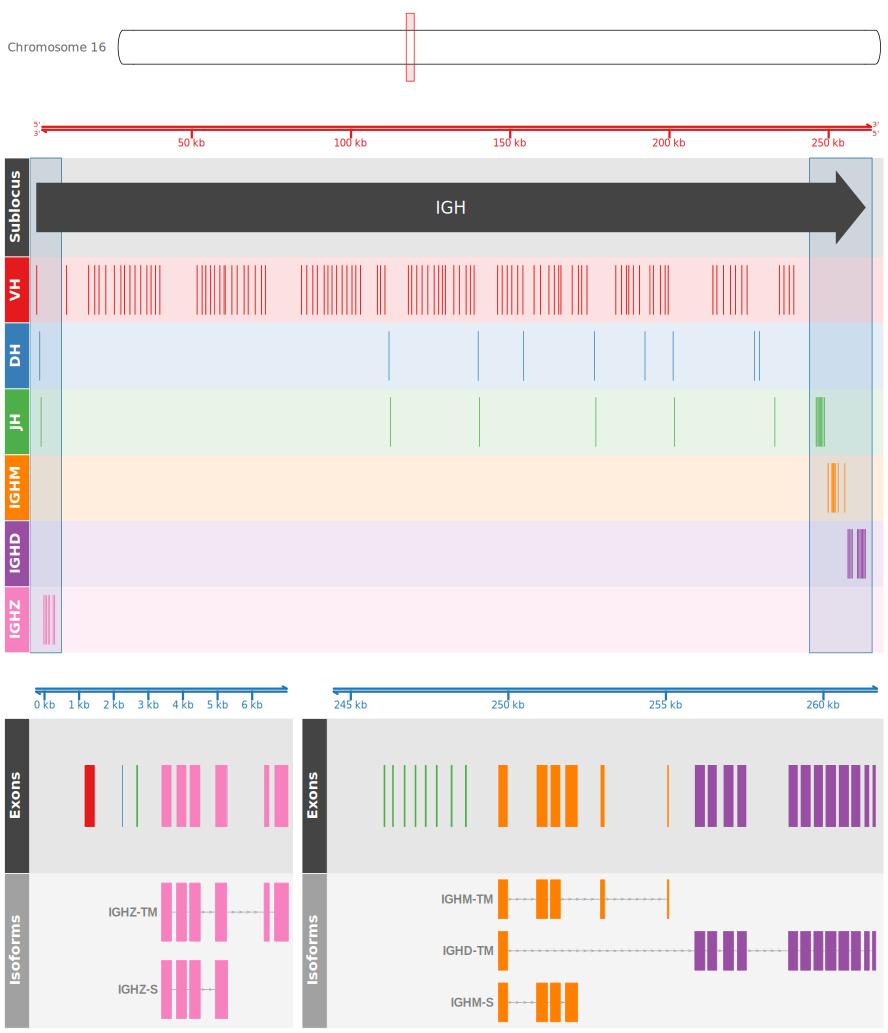
\includegraphics[width=\textwidth]{/home/will/Documents/code/figures/2018-11-07/xma-locus-map} % TODO: Move to thesis directory, switch to large version
	\caption[The immunoglobulin heavy chain (\textit{IGH}) locus in \textit{}]{\textbf{The immunoglobulin heavy chain (\textit{IGH}) locus in \textit{Xiphophorus maculatus}:} (A) Position of the \textit{IGH} locus on chromosome (group) 16 of the \textit{X. maculatus} genome. (B) Arrangement of VH, DH, JH and constant-region gene segments on the \textit{X. maculatus} \textit{IgH} locus. (C) Detailed map of the \textit{IGHZ} and \textit{IGHM/D} constant regions, indicating the position and identity of the constant-region exons and the exon composition of expressed \textit{IgH} isoforms in \textit{X. maculatus}.}
	\label{fig:xma-locus-map}
	\end{figure}
	
		\begin{figure}
	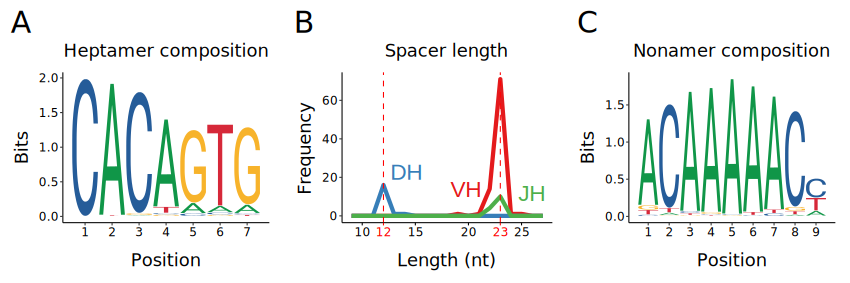
\includegraphics[width=\textwidth]{_Figures/png/xma-rss-seqlogo-all}
	\caption[Recombination signal sequences in the \textit{X. maculatus} \textit{IGH} locus]{\textbf{Recombination signal sequences in the \textit{X. maculatus} \textit{IGH} locus:} (A) Sequence composition of conserved heptamer sequences across all \textit{X. maculatus} heavy-chain RSSs; (B) length distribution of unconserved spacer sequences in \textit{X. maculatus} heavy-chain RSSs; (C) sequence composition of conserved heptamer sequences across all \textit{X. maculatus} heavy-chain RSSs.}
	\label{fig:xma-rss-seqlogo-all}
	\end{figure} % TODO: Add in row showing expected consensus sequence with highlighted conserved positions

	


	\subsection{Variable regions}
	
			\begin{figure}
	\centering
	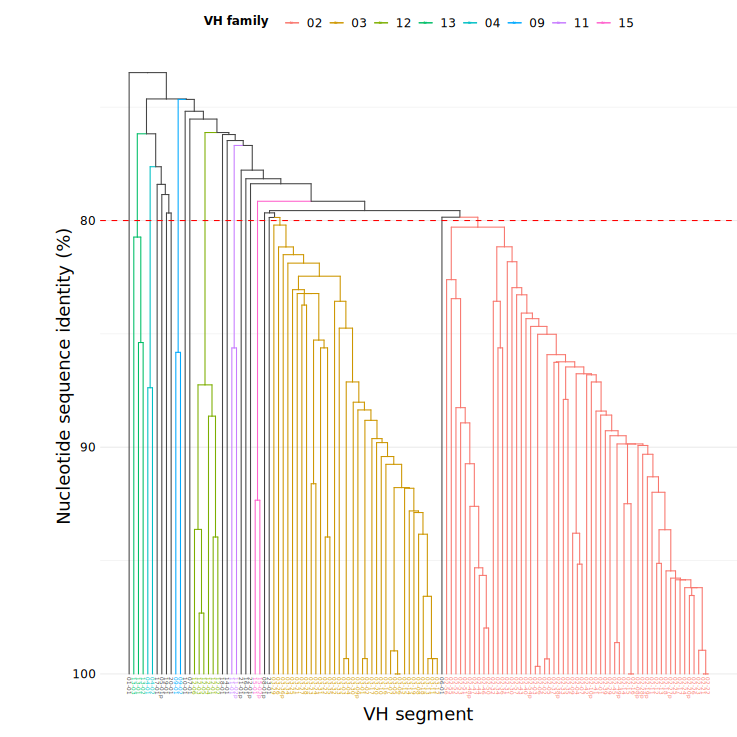
\includegraphics[width=\textwidth]{_Figures/png/xma-vh-families-tree} % TODO: Move to thesis directory, switch to large figure
	\caption[VH families in the in \textit{X. maculatus} \textit{IgH} locus]{\textbf{VH families in the in \textit{X. maculatus} (\textit{IgH}) locus:} (A) Dendrogram of sequence similarity of VH segments in the \textit{X. maculatus} locus, arranged by single-linkage clustering on nucleotide sequence identity. The red line indicates the 80\% cutoff point for family assignment. (B) Sequence identity table for \textit{X. maculatus} VD segments, with similarity levels exceeding the familial threshold highlighted in red. Grey boxes indicate family relationships among segments. In both subfigures, VH segment names from the IGH1 sublocus are displayed in black, while IGH2 VH segments are displayed in blue.}
	% TODO: Fix up this figure
	\label{fig:xma-vh-families-tree}
	\end{figure}
	
				\begin{figure}
	\centering
	\includegraphics[width=\textwidth]{_Figures/png/xma-vh-families-map} % TODO: Move to thesis directory, switch to large figure
	\caption[VH families in the in \textit{X. maculatus} \textit{IgH} locus]{\textbf{VH families in the in \textit{X. maculatus} (\textit{IgH}) locus:} (A) Dendrogram of sequence similarity of VH segments in the \textit{X. maculatus} locus, arranged by single-linkage clustering on nucleotide sequence identity. The red line indicates the 80\% cutoff point for family assignment. (B) Sequence identity table for \textit{X. maculatus} VD segments, with similarity levels exceeding the familial threshold highlighted in red. Grey boxes indicate family relationships among segments. In both subfigures, VH segment names from the IGH1 sublocus are displayed in black, while IGH2 VH segments are displayed in blue.}
	% TODO: Fix up this figure
	\label{fig:xma-vh-families-map}
	\end{figure}



	\subsection{Constant regions}
	
		\begin{figure}
	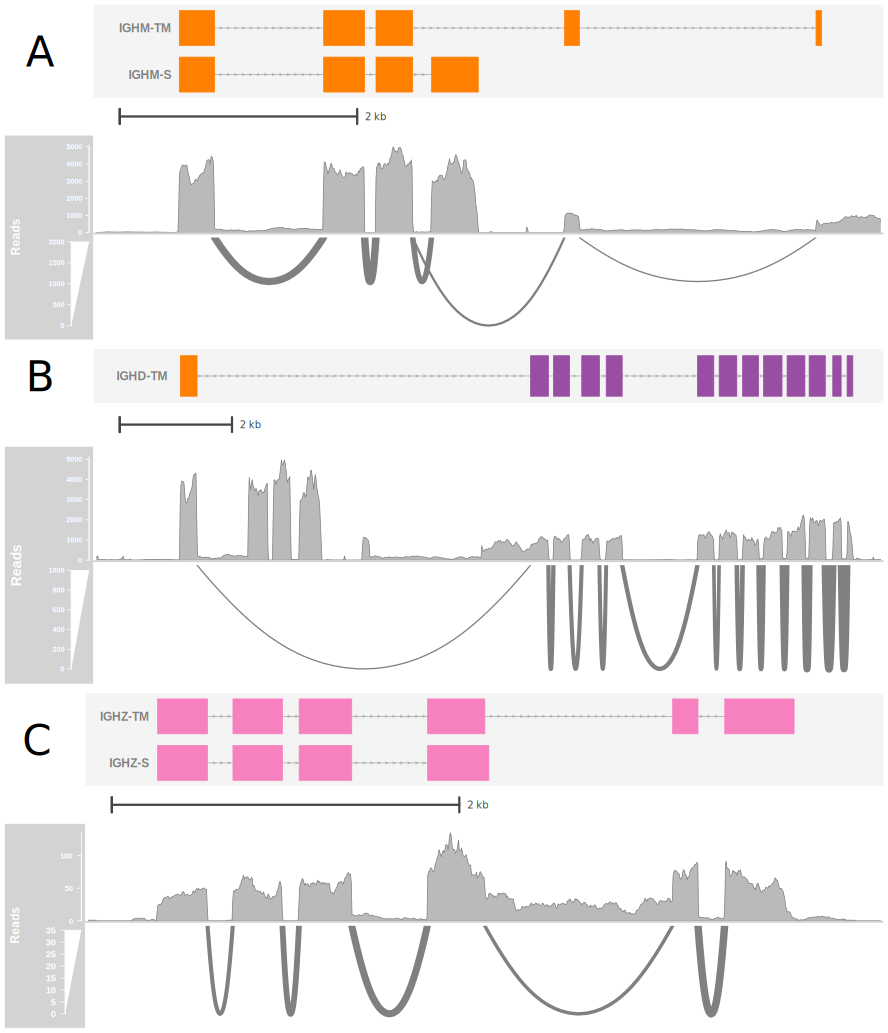
\includegraphics[width=\textwidth]{_Figures/png/xma-locus-sashimi}
	\caption[Constant-region isoforms in \textit{X. maculatus}]{\textbf{Constant-region isoforms in \textit{X. maculatus}:} Coverage and sashimi plots of STAR-aligned RNA-seq reads from \textit{X. maculatus} samples, demonstrating the splicing behaviour of IGH1 constant-region isoforms. (A) IGHM exon splicing, showing alternative splicing patterns of IGHM-TM and IGHM-S; (B) IGHD exon splicing, including splicing of \cm{1} to \cd{1}; (C) IGHZ exon splicing.}
	\label{fig:xma-locus-sashimi}
	\end{figure}


\section{Comparitive analysis of \textit{IgH} constant-region structure in the Cyprinodontiformes}

	\subsection{Evolutionary history of IgZ}
	
	\subsection{Sublocus multiplicity and orientation}
	
	\subsection{Exon usage in transmembrane IgM \& other isoforms}






%\section{The combination of genome and BAC data reveals a two-part sublocus on chromosome 6}
%
%The structure of the immunoglobulin heavy chain (IgH) locus provides the fundamental underpinning of antibody diversity in a species, defining the space of possible sequences arising from the VDJ recombination process, the functional antibody classes available via the constant-region exons, and the possible splicing behaviour of those exons. In order to investigate the dynamics of antibody immunity in a species, it is therefore necessary to have at least a working knowledge of its IgH structure, and ideally a comprehensive characterisation. Such a characterisation provides both the primer sequences required for immunoglobulin sequencing and the complete V, D and J-segment databases required for analysis of Ig-seq data, as well as directly providing information about antibody immunity in a species.
%
%In order to obtain such a characterisation for the turquoise killifish, I sequenced and assembled several  clones from the TK bacterial artificial chromosome (BAC) library suspected to contain parts of the locus. (see \dots for details on the BAC assembly method). In parallel, I collated comprehensive VH, JH and CH-exon sequence databases for three model teleost species with previously assembled IgH loci: zebrafish (\textit{Danio rerio} \citep{} ), stickleback (\textit{Gasterosteus aculeatus} \citep{}) and medaka (\textit{Oryzias latipes} \citep{} ). These databases were aligned against the most recent assembly of the TK genome (\dots) to identify scaffolds potentially bearing part of the IgH locus. Finally, the BAC inserts and genome scaffolds were aligned together to produce a single, contiguous locus sequence.
%
%In total, one chromosome (chr6) and four smaller scaffolds were identified as bearing probable IgH locus fragments (\Cref{tab:nfu_locus_scaffolds}). The existing chromosome 6 assembly contained what appeared to be a complete (V-D-J-CM-CD) sublocus on the sense strand, as well as a single downstream VH segment in antisense; the presence and position of this inverted V suggested the presence of at least one more sublocus, present in antisense downstream of the already-assembled sublocus, which had not been included in the chromosome assembly. % Other identified scaffolds
%
%Taken together, these data suggested a model of the TK IgH locus in which two apparently-complete subloci face each other on opposite strands of chromosome 6. This hypothesis was confirmed by the BAC assembly data, which confirmed the existence of at least two non-overlapping subloci with distinct VH structures. The first of these, from the aligned inserts of several BACs including \dots, shows high identity with the 5' sense-strand sublocus present on chromosome 6, while the second, contained in the inserts of BACs \dots, aligns with scaffolds \dots and the inverted VH region on chromosome 6, with the \dots insert extending into the post-IgH 3' part of the chromosome. % Figure for this?
%Integrating all these data gave rise to the contiguous locus sequence outlined in \dots. %figure
%
%As is the case in most teleosts, but unlike in salmonids, only a single IgH locus could be identified; the two genome scaffolds that could not be integrated into the locus sequence contained either VH and JH or VH sequences only, and appear to represent orphaned variable-region segments rather than a functional second locus. No other chromosome was found to contain a multi-part, contiguous sequence resembling that found on chromosome 6. 
%
%In conclusion, the African turquoise killifish genome contains a single immunoglobulin heavy-chain gene locus, approximately 305 kilobases in length. This sequence appears to contain exactly two structurally-complete subloci, present in tandem but on opposite strands, each containing VH, DH (see below), JH and constant-region sequences. The structural completeness of both subloci suggest that both may be capable of recombining to produce functional IgH transcripts; \dots % Functionality of antisense sublocus?
%
%% NB: It would be really nice to get single-cell DNA sequencing of killifish B-cells and see if there are any cells where both subloci are recombined; do you maybe get more than one chance per chromosome?
%
%\begin{table}
%\begin{threeparttable}
%\begin{tabular}{ccccccc}\toprule
%Scaffold & Total length (kb) & V & J & \cm{} & \cd{} & \cz{} & Included in locus?\\
%chr6 & 6195.6 & 15 & 7 & 5 & 11 & Yes\\
%scf10901 & 1.4 & 0 & 0 & 0 & 3 & Yes\\
%scf35954 & 16.3 & 3 & 0 & 0 & 0 & No\\
%scf36277 & 18.9 & 2 & 1 & 0 & 0 & No\\
%scf9157 & 7.2 & 0 & 7 & 4 & 0 & Yes\\
%\end{tabular}
%\caption{Summary of genome scaffolds containing putative \textit{IgH} locus fragments}
%\end{threeparttable}
%\label{tab:nfu_locus_scaffolds}
%\end{table}
%
%\begin{figure}
%\caption{Assembly of the \textit{N. furzeri} \textit{IgH} locus sequence from genome scaffolds and BAC inserts.} 
%\end{figure}
%
%\section{}
%
%% Similarity between IGH1 and IGH2 (esp D, J, constant regions - but not V?)
%
%Having generated a contiguous sequence for the IgH locus, constant-region exons from the three reference species were realigned to the new locus in the same manner they had been aligned to the genome and BAC sequences previously. These alignments were used as the basis for detailed characterisation of CH exons in the TK locus. To refine intron/exon boundaries and analyse splicing behaviour, RNA-seq data from eight mature killifish (GRZ-Bellemans, 4 $\times$ 6-week-old fish, 4 $\times$ 16-week-old) was mapped to the locus with STAR (\dots methods link here, inc. repeat-masking \dots); the combination of a B-cell-rich source tissue (\dots citation needed \dots) and the use of data from several individuals enabled clear delineation of intron/exon boundaries, as well as identification of the second transmembrane exon for both IgM and IgD in both subloci. % Example figure?
%
%The exon structure of both subloci is identical, though there are some differences in spatial arrangement: in IgH2, for example, the 5' and 3' IgD exons are separated by a large \dots region which is absent in IgH1. The exon sequences of the two subloci is also very similar, with an average of \dots \% sequence identity between corresponding exons. % Does this tell us anything about the duplication timing?
%Given this high level of similarity in sequence and exon arrangement, it is perhaps unsurprising that the splice patterns of the two subloci appear to be identical % Though, many reads will be mapping to both
